% "Станет проще"

\documentclass[a4paper,12pt]{article} % тип документа

% report, book

%  Русский язык

\usepackage[T2A]{fontenc}			% кодировка
\usepackage[utf8]{inputenc}			% кодировка исходного текста
\usepackage{graphicx}
\usepackage[english,russian]{babel}	% локализация и переносы


%отступ
\usepackage[left=3cm,right=3cm,
    top=2cm,bottom=2cm,bindingoffset=0cm]{geometry}

% Математика
\usepackage{amsmath,amsfonts,amssymb,amsthm,mathtools} 
\usepackage{csvsimple}
\usepackage{multirow}

\usepackage{hyperref}
\usepackage{wasysym}
\usepackage{subcaption}
\usepackage{verbatim}
\usepackage{hyperref}
\usepackage{float}
\usepackage{enumerate}
\usepackage[dvipsnames]{xcolor}
%Заговолок
\graphicspath{ {img/} }


\begin{titlepage}
\author{Соловьянов Михаил }
\title{Задание 13. Вектора. Потенциал.}
\date{\today}
\end{titlepage}



\begin{document} % начало документа
\maketitle
%http://easyfizika.ru/zadachi/elektrostatika/



\textit{Указание: Задачи оформлять ссылаясь на физические законы которые применяются для их решения.}




\section{Вектора (математика)}
\begin{enumerate}

	\item Прочитать про вектора в физике тут !` \url{https://mathus.ru/phys/vectors.pdf} !!! Копия так же представлена в репозитории ( /lib/math/vectors.pdf) 

	\item Найти и изучить видео по векторам и их произведениям.

	\item Дан параллелограмм $ ABCD $ . Диагонали $AC $ и $ BD $ пересекаются в точке $ O $ . Пусть , $ \vec{AB} = \vec{a} $ , \vec{AD} = \vec{b} $ , тогда \vec{OA} = x\vec{a} + y\vec{b} $ , где $ x$  и $y $ – некоторые числа. Найдите число, равное $ x + y$.


	\begin{figure}[H]
	\centering
	  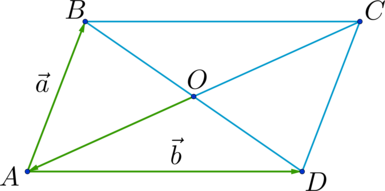
\includegraphics[width=0.5\linewidth]{vector1.png}
	  \caption{ }
	  \label{task1}
	\end{figure}

	
	\item  Найти разность векторов $ \vec{a} = \{1; 2\} $ и  $\vec{b} = \{4; 8\}$.


	\item Найти сумму векторов  $ \vec{a}= \begin{bmatrix}1\\ 2 \\ 5 \end{bmatrix} $ и $ b = \begin{bmatrix}4\\ 8 \\ 1 \end{bmatrix}$. 

	\item Найти сумму векторов  $ \vec{a} = \begin{bmatrix}2\\ 0 \\ \frac{1}{4} \\ 7 \end{bmatrix} $ и $ \vec{b} = \begin{bmatrix}19\\ 3 \\ 1 \\1 \end{bmatrix}$. 


	\item Найти разность векторов $\vec{a} = \{1; 2; 5; -1; 5\}$ и $\vec{b} = \{4; 8; 1; -1; 2\}$. 

	


	\item Прочитать про скалярные произведения тут !!! \textbf{ \url{https://dep805.ru/education/portal/5/laag/laag4.pdf}} !!! Копия так же представлена в репозитории ( /lib/math/...)


	\item Как вы понимаете практический смысл скалярного произведения??




	\item Найти скалярное произведение векторов $\vec{a}$ и $\vec{b}$, если их длины $|a| = 3$, $|b| = 6$, а угол между векторами равен $ \pi / 3 $. 

	\item Найти скалярное произведение векторов $\vec{a}$ и $\vec{b}$, если их длины $|a| = 1.5$, $|b| = 1.2$, а угол между векторами равен $ 90 $ градусов. 

	\item Найти скалярное произведение векторов $\vec{a}$ и $\vec{b}$ если:

	 \begin{enumerate}

	 	\item $\vec{a} = \{1; 2\}$ и $\vec{b} = \{-1; 2\}$.

	 	\item $\vec{a} = \{0; 1\}$ и $\vec{b} = \{-1; 0\}$.

	 	\item $\vec{a} = \{10; 2\}$ и $\vec{b} = \{-2; 2\}$.

	 	\item $ \vec{a} = \begin{bmatrix}2\\ 0 \\ \frac{1}{4} \\ 7 \end{bmatrix} $ и $ \vec{b} = \begin{bmatrix}19\\ 3 \\ 1 \\1 \end{bmatrix}$. 


	 \end{enumerate} 
\end{enumerate}


\section{Напряженность}
\begin{enumerate}


	\item Дана металлическая сфера радиусом $ R_1 $ с полостью внутри радиуса $ R_2 $. Пусть сфера помещена в равномерное поле напряженностью $ \vec{E} $ чему равна напрженность в центре сферы? Ответ обосновать.


	\item Из файла \textit{/lib/fizika20191028proba5+otvet.pdf}  репозитория решить задачи 14,16 первого варианта. 

\end{enumerate}



\section{Потенциал}
\begin{enumerate}


\item Чтобы в воздухе при атмосферном давлении проскочила искра, в нём должно быть электростатическое поле, модуль напряжённости которого не менее $ \vec{E} = 6,00 $ МВ/м . Определите разность потенциалов между облаком и поверхностью Земли во время грозы, если длина «искры» — молнии — $ d=200 $ м.

\item В вершинах равностороннего треугольника со стороной $ a=2 $ см расположены точечные заряды $  Q=2 $ мкКл. Какую работу нужно совершить, чтобы переместить точечный заряд  $ q=5 $ нКл из середины одной из сторон треугольника в его центр?

\item Расстояние между точечными зарядами $ q_1=10 $ нКл и  $ q_2=-1 $ нКл равно $r=1,1$ м. Найдите напряженность поля в точке на прямой, проходящей через заряды, в которой потенциал равен нулю.

\end{enumerate}



\section{Материалы}

\paragraph{Про скалярное произведение читать тут:}\\ 
\url{https://dep805.ru/education/portal/5/laag/laag4.pdf}


\end{document}